% Address the question: What problem are you solving, or opportunity are you seizing? 
% \section{1 intro}
% \firstsection{Introduction}
% In times of global pandemics that require e
 % is highly desirable

Effective remote collaboration is facilitated by increasing the (psychological) depth of people's remote connections. One requirement for truly connected experiences is the strength of immersion into virtual environments. Room-scale VR significantly increases the users immersion by, first and foremost, allowing free movements, simulating \textit{natural} real world sensory experiences due to locomotion. Further, synchronized motion capture allows avatar movements to be rendered to represent ones own body movements. In VR, several illusions, such as the place-- and plausibility illusions,  occur at the same time and are prerequisites for the user to feel present. Depending on the effectiveness of the employed illusions and whether multiple illusions work congruently, participants experience a feeling of presence in VR~\cite{Gonzalez-Franco2017, Kilteni2012}. Such illusions enrich and/or modify participants subjective experience in VR. Together, free movement, \textit{realistic} avatar rendering, and contextual components of the VR experience coincide at the same time for the user to feel present. Therefore, designing immersive experiences for room-scale VR aims at facilitating the emergence of presence experience, ultimately providing the foundation for genuinely connected remote social experiences.

% Most prominently, the embodiment illusion, or body ownership transfer, has proven to elicit \textit{realistic} behavioral as well as physiological responses, when a strong emotional stimulus such as virtual hurting of an embodied rubber hand is given. 

% \section{2 Parametric Maps to investigate user behavior and Experience}
\section{Parametric Maps to investigate user behavior and Experience}

In order to scale immersive VR technology to a broader public with use cases ranging from remote office work to entertainment, inclusive design principles are of key importance to successfully design presence experience across a wide user base. Individual differences, for example the eagerness to physically move through virtual worlds, significantly challenge designing for presence experience, thereby challenging acceptance of VR technology in general~\cite{Sagnier2020}. Here, designers and developers would benefit from a better understanding of user behavior, being able to directly query the impact of certain characteristics of the user base. Specifically in room-scale VR applications, leveraging inherent motion capture provides the opportunity for a data-driven understanding of user behavior with a high spatial resolution. Spatial resolution here pertains to using motion capture data from room-scale VR to specify, for example, how much time the user spends at any given location in virtual space and how much of this behavior can, for example, be explained by the users' previous video game experience. However, many studies commonly consider aggregated data missing the opportunity to spatially resolve effects of interest.

% \begin{figure*}[!ht]
% \centering
% 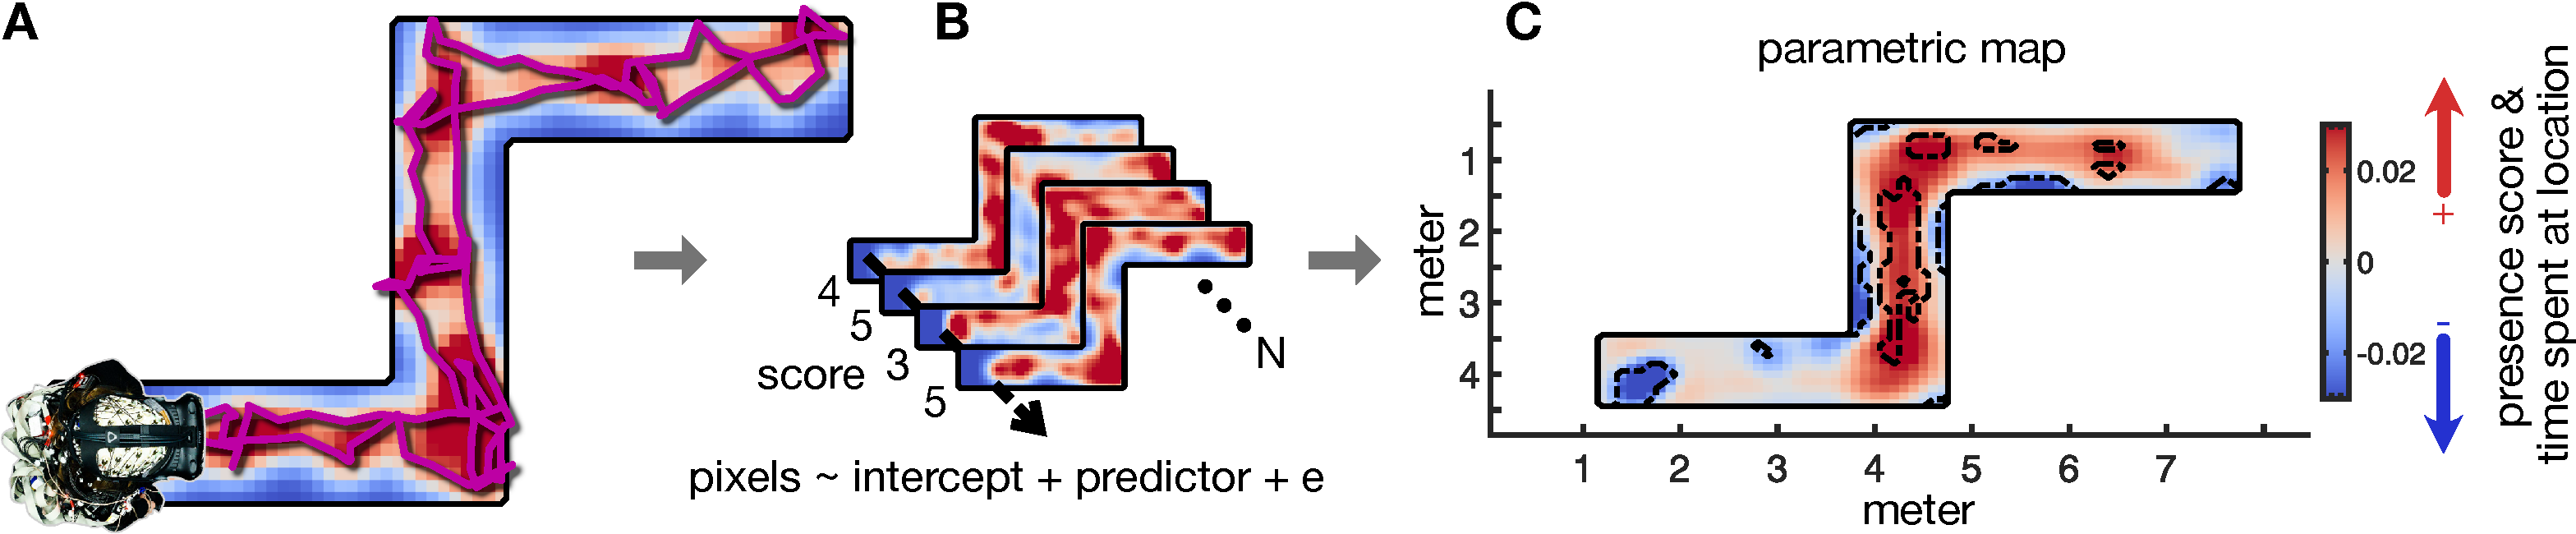
\includegraphics[width=\linewidth]{figures/fig1.pdf}
% \vspace{6pt}
% \caption{We propose parametric maps to study user behavior and experience and guide future design of room-scale VR applications. \textbf{A,} Top-down view on the participant equipped with a wireless VR headset and backpack PC at the start of a `Z' maze. Motion capture of exploration paths (solid pink line) was spatially blurred using a Gaussian filter to obtain images/maps in B suited for across participants analyses of moderating variables. \textbf{B,} We constructed parametric maps of where participants spent time exploring the mazes as a function of their experienced presence. \textbf{C,} We found that with increasing presence, participants were more likely to stay in the center of the paths as well as in segments \textit{presumably} critical for navigational success. Significant pixels at $p<0.05$ are masked with a dotted line}
% \label{fig:methods}
% \end{figure*}

In this methodological research contribution, we propose parametric maps as a way to study user behavior, and ultimately user experience, utilizing the inherent motion capture of current VR hardware that provides high resolution regarding the users' movement in virtual space. Specifically, we demonstrate using general linear model, \textit{GLM}, in a mass-univariate application that allows linear decomposition of user behavior across all pixels of a given room-scale VR space. GLM encompasses familiar statistical models, like linear regression and ANOVA as well as ANCOVA. It allows for \textit{t}-tests and variance ratio tests, i.e. \textit{F}-tests. Further, the approach is scalable to additional models in the broad \textit{GLM family} therefore providing a framework with significant flexibility. The proposed analyses scheme is easily extendable to 3D space, i.e. voxels, for example to investigate individual differences in manual interaction scenarios.

Following below, we demonstrate the proposed analyses scheme showing how differences in subjectively reported experienced presence impacts participants movement profiles in a \textit{beyond} room-scale VR spatial exploration task. However, we situate our approach specifically as a tool for statistical assessment of spatially resolved multimodal data streams in the related works section as we believe it best highlights the usefulness of the method. Then, we guide the reader in a step-by-step fashion through the pre-processing, model fitting, and inference steps in order to construct \textit{parametric maps}. To highlight potential benefits when considering individual characteristics, we close with a linear regression scheme predicting presence via individual characteristics.